\documentclass{article}

\usepackage{algorithmic}
\usepackage{amsmath}
\usepackage{graphicx}
\usepackage{hyperref}
\usepackage{booktabs}

\begin{document}

\title{Naive Bayes Handwriting Recognition}
\author{Geoffrey Ulman\\
        Homework 7\\
        CSI873}
\date{November 2011}
\maketitle

\section{Results}\label{Results}

A testing error rate of \(0.388\) and a training error rate of \(0.322\) was acheived by the Naive Bayes classifier with 95\% confidence intervals given by Table \ref{error}. On a digit-by-digit basis, error was relatively uniform among the digits, with ``4'' and ``5'' being significant exceptions (see Figure \ref{trainconfusion} for the training data confusion matrix and Figure \ref{testconfusion} for the testing data confusion matrix). In the case of ``5'' missclassifications were spread over a number of digits. In the case of ``4'' almost all the missclassifications were missclassifying ``4'' as ``9'' (see Figures \ref{4_9_missclass_training} and \ref{4_9_missclass_training}).

\begin{figure}
\centering
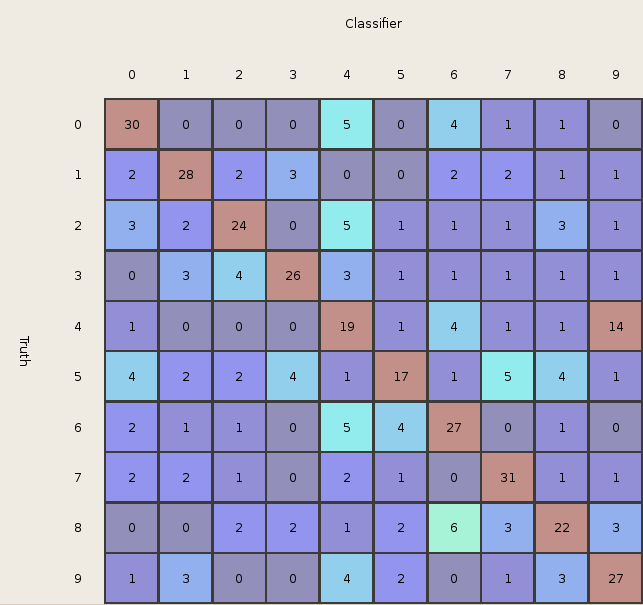
\includegraphics[width=0.7\textwidth]{ConfusionMatrixTesting.png}
\caption{Confusion Matrix for Testing Data Set}
\label{testconfusion}
\end{figure}

\begin{figure}
\centering
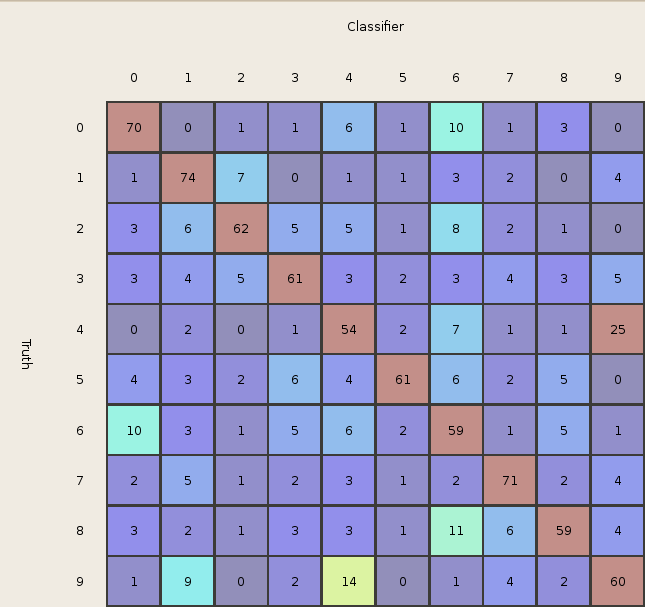
\includegraphics[width=0.7\textwidth]{ConfusionMatrixTraining.png}
\caption{Confusion Matrix for Training Data Set}
\label{trainconfusion}
\end{figure}

\begin{figure}
\centering
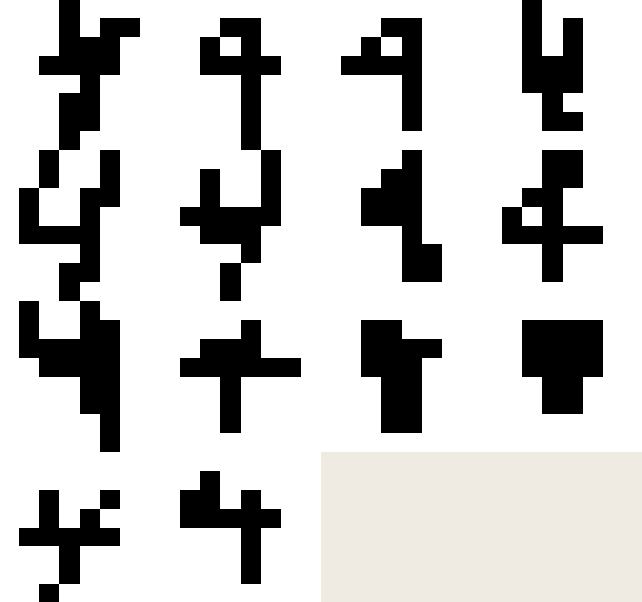
\includegraphics[width=0.7\textwidth]{4-9-testing.png}
\caption{4s Misclassified as 9s in Testing Data Set}
\label{4_9_missclass_training}
\end{figure}

\begin{figure}
\centering
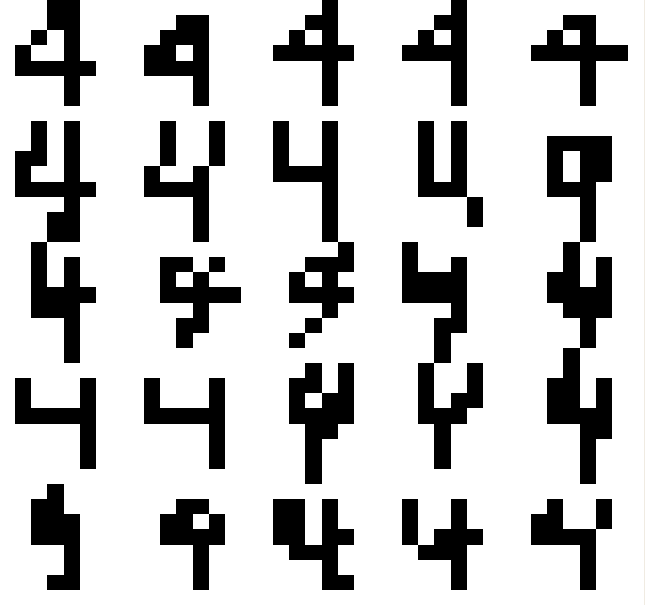
\includegraphics[width=0.7\textwidth]{4-9-training.png}
\caption{4s Misclassified as 9s in Training Data Set}
\label{4_9_missclass_training}
\end{figure}

\begin{table}
\caption{Misclassification Error}
\begin{center}
\begin{tabular}{llcc}
\toprule
Data Set & Error & \multicolumn{2}{c}{95\% Confidence Interval} \\
\cmidrule(r){3-4}
& & Lower Bound & Upper Bound \\
\midrule
Testing       & 0.388 &  0.341 & 0.435  \\
Training      & 0.322 &  0.291 & 0.352  \\
\bottomrule
\end{tabular}
\label{error}
\end{center}
\end{table}

\begin{thebibliography}{9}

\bibitem{cpl}
  Tom M. Mitchell,
  \emph{Machine Learning},
  WCB McGraw-Hill, Boston,
  1997.

\end{thebibliography}

\end{document}
